\section{长短时记忆网络}
\label{sec:lstm}

\begin{frame}
  \begin{center}
    \Huge{\textcolor{red}{长短时记忆网络}}
  \end{center}

  \begin{enumerate}
    \item \alert{网络架构}
    \item \alert{网络变种}
  \end{enumerate}
\end{frame}

\subsection{架构}

\begin{frame}[fragile]{网络架构}
  \begin{figure}
    \centering
    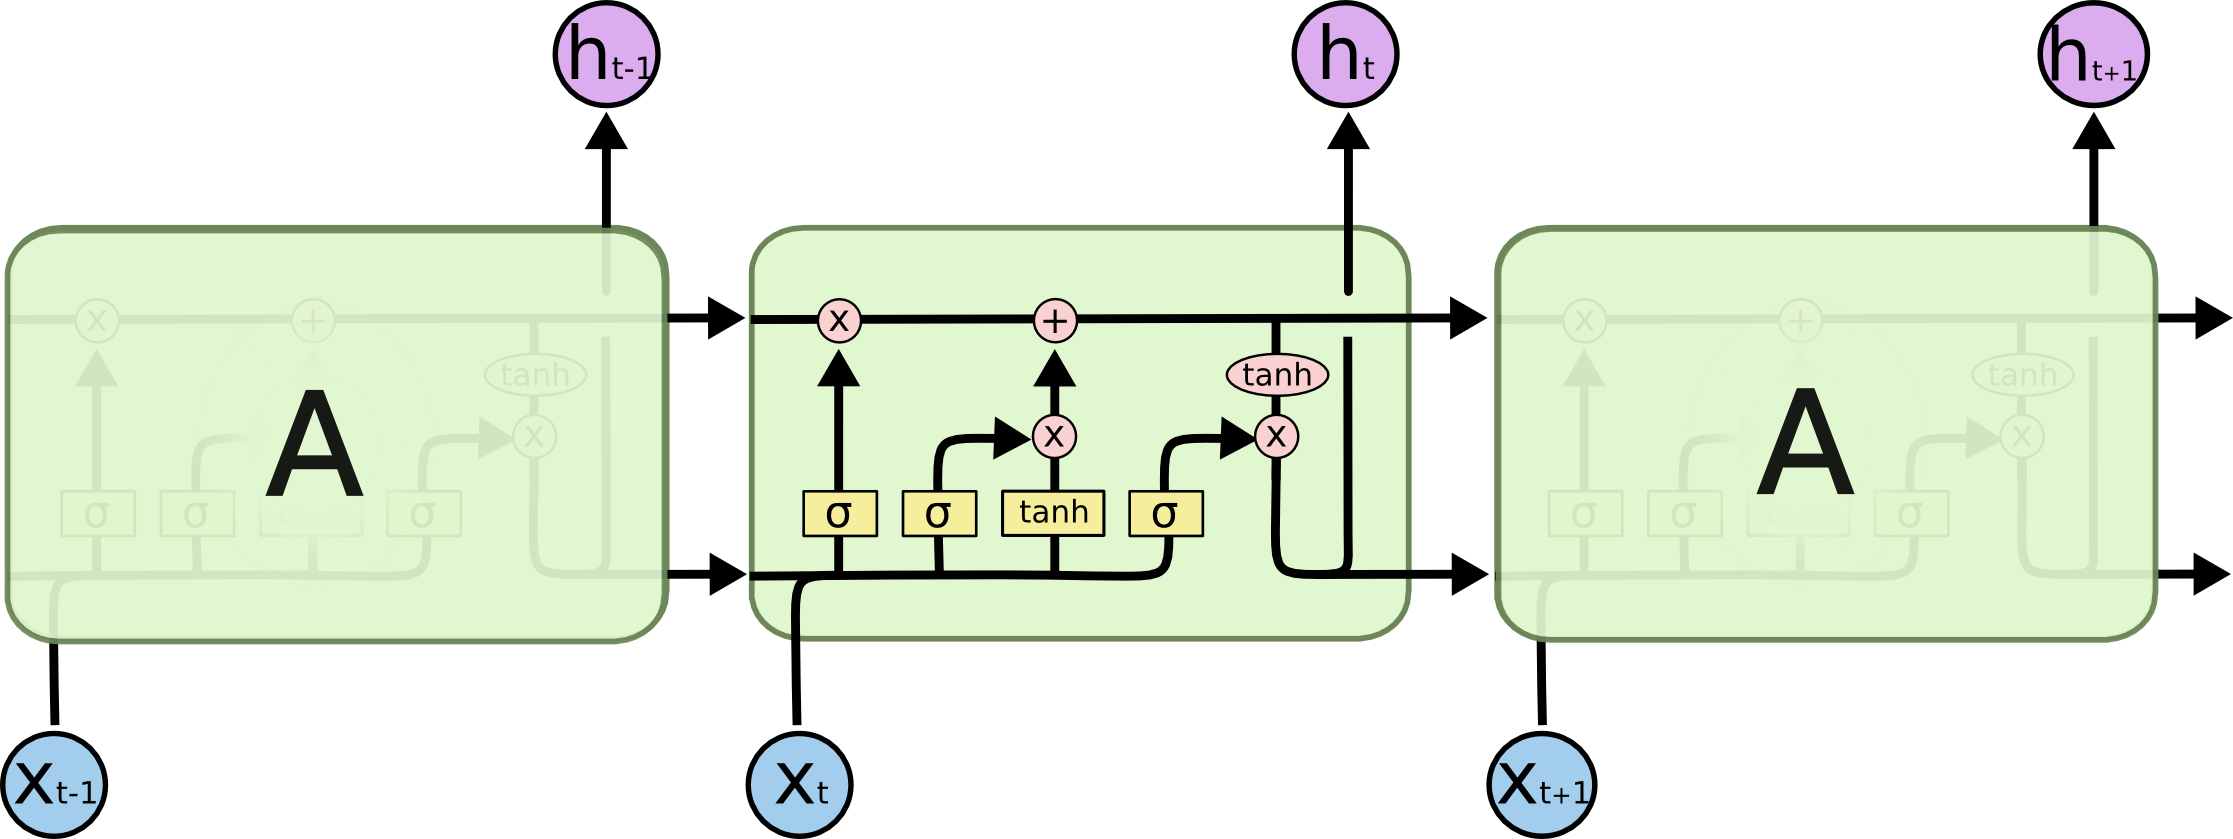
\includegraphics[width=0.9\textwidth]{LSTM3-chain.png}
  \end{figure}
\end{frame}

\begin{frame}[fragile]{遗忘门}
  \begin{figure}
    \centering
    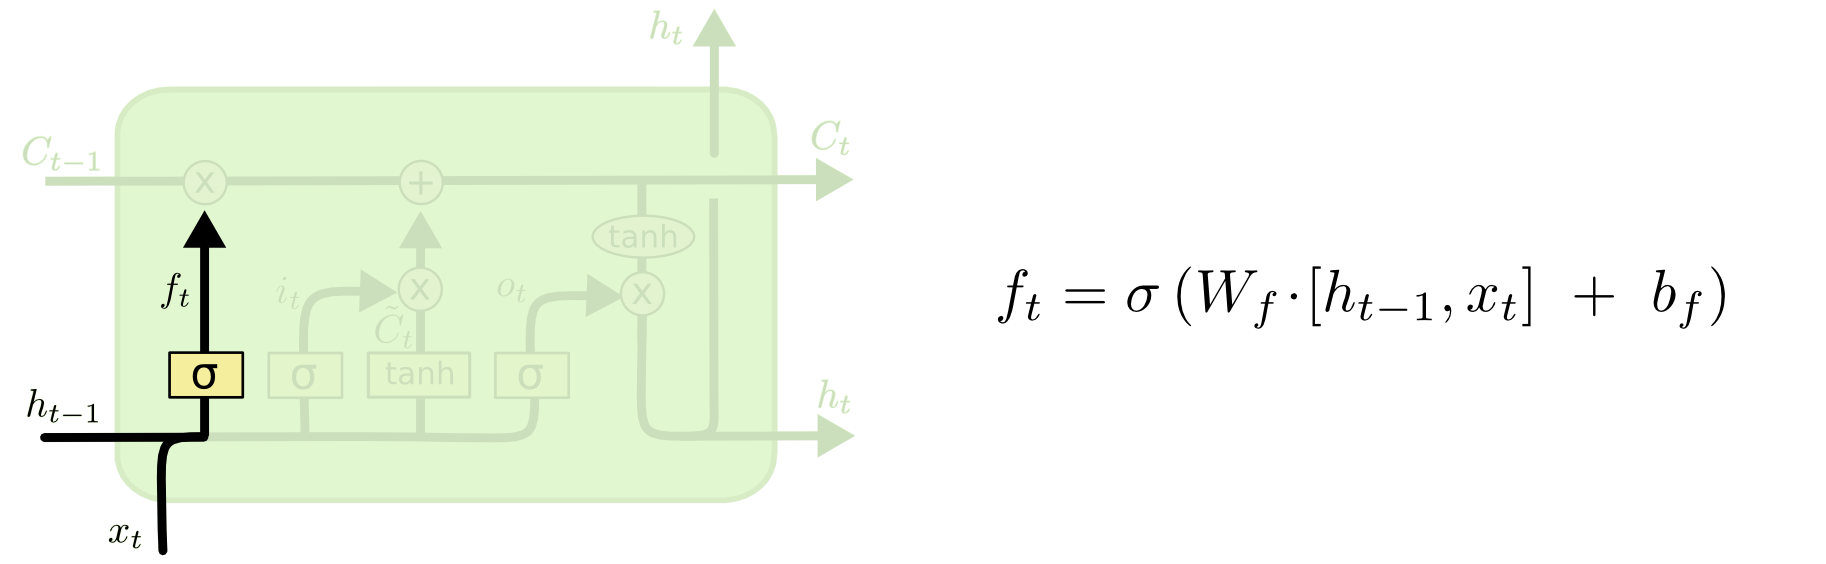
\includegraphics[width=0.9\textwidth]{LSTM3-focus-f.png}
  \end{figure}
\end{frame}

\begin{frame}[fragile]{输入门}
  \begin{figure}
    \centering
    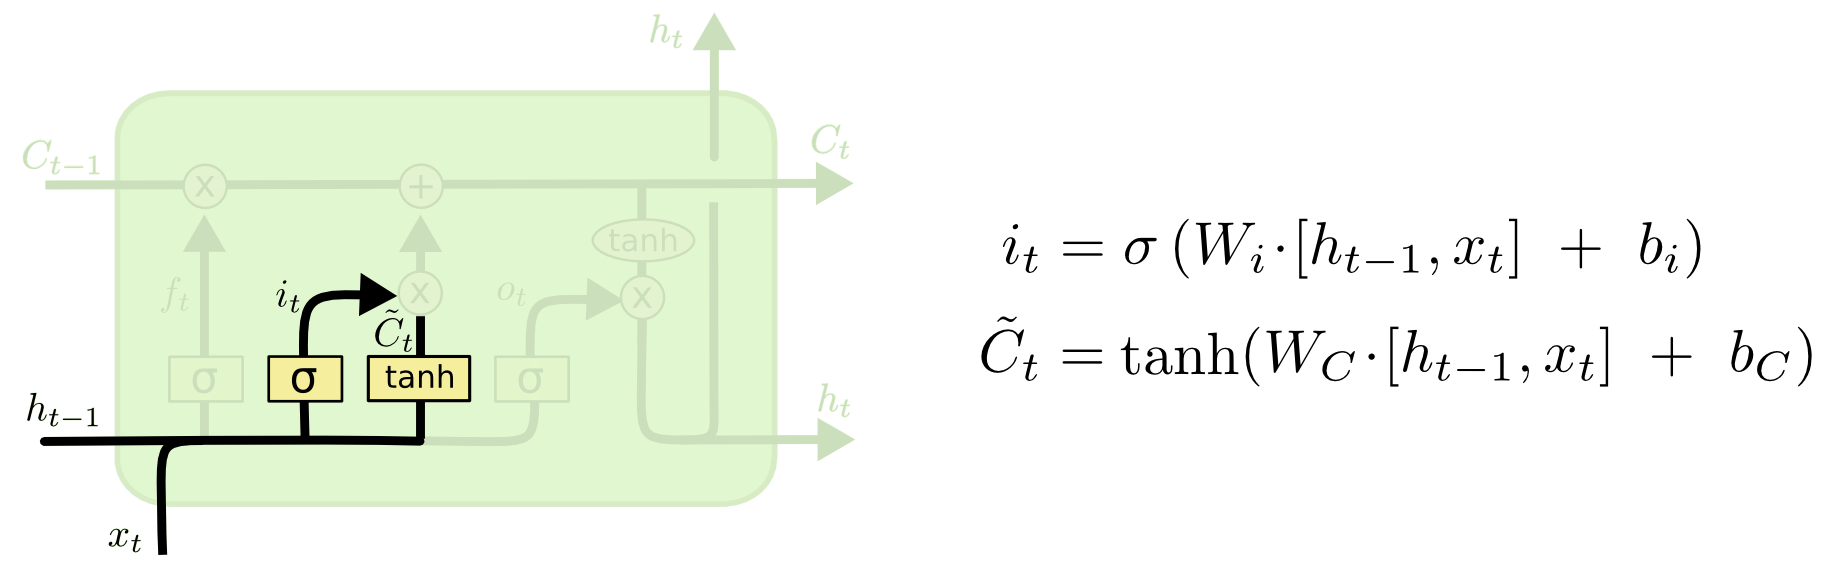
\includegraphics[width=0.9\textwidth]{LSTM3-focus-i.png}
  \end{figure}
\end{frame}

\begin{frame}[fragile]{输出门}
  \begin{figure}
    \centering
    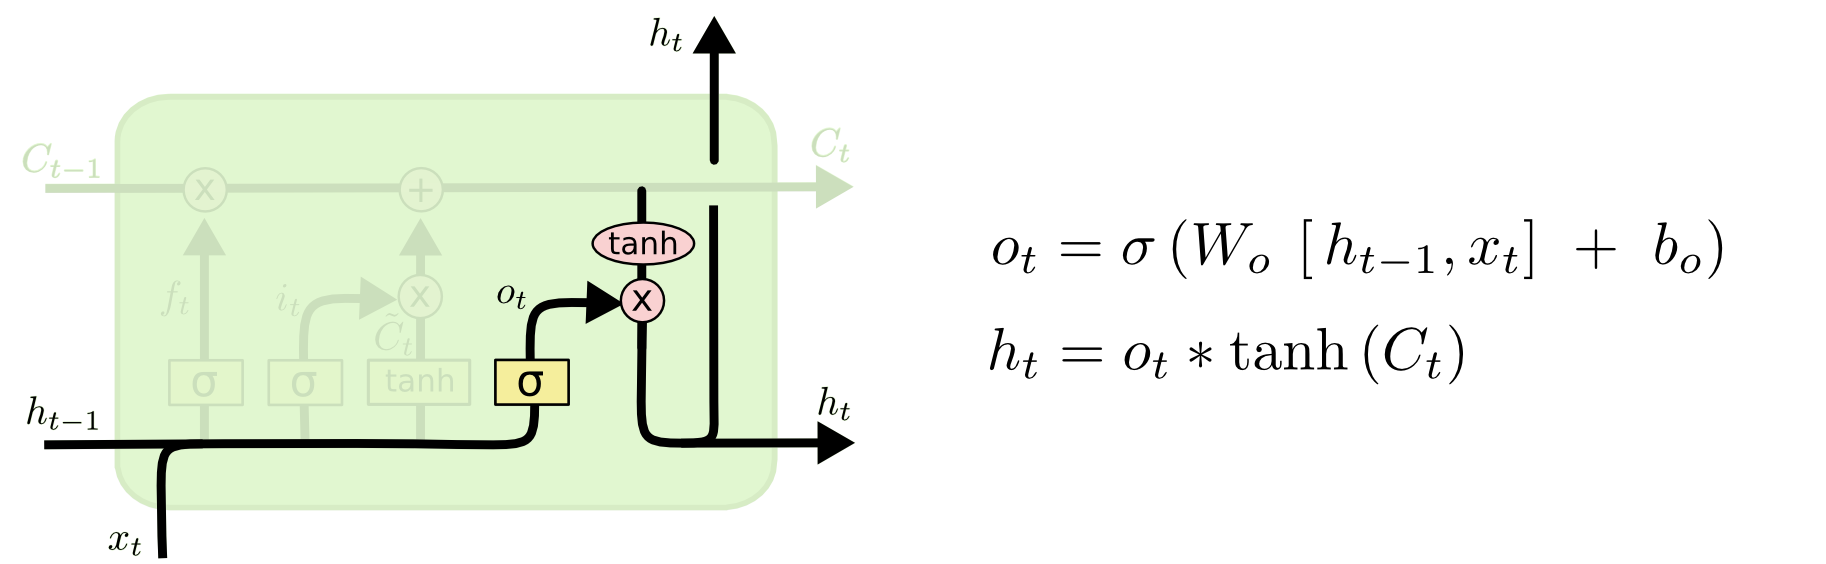
\includegraphics[width=0.9\textwidth]{LSTM3-focus-o.png}
  \end{figure}
\end{frame}

\subsection{计算}

\begin{frame}[fragile]{初始状态: $t-1$时刻}
  \begin{figure}
    \centering
    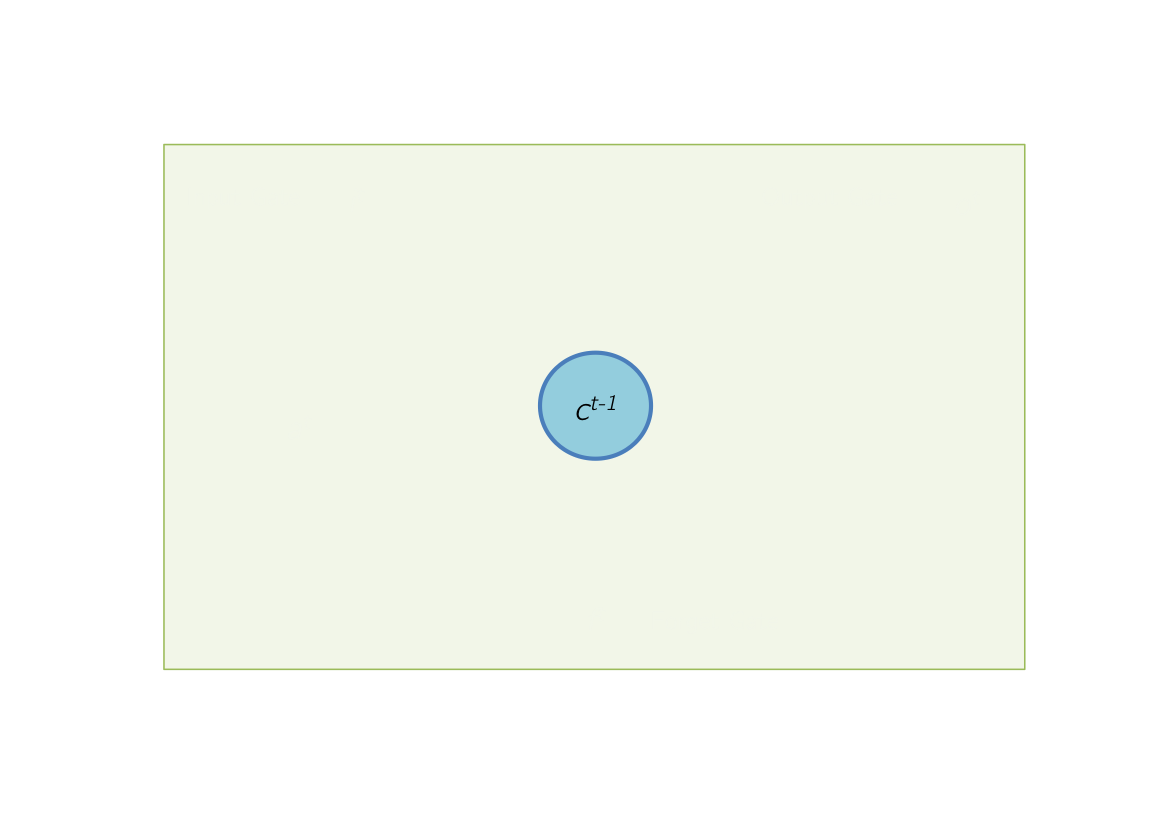
\includegraphics[width=0.8\textwidth]{lstm-init.png}
  \end{figure}
\end{frame}

\begin{frame}[fragile]{前向传播:输入与门计算}
  \begin{figure}
    \centering
    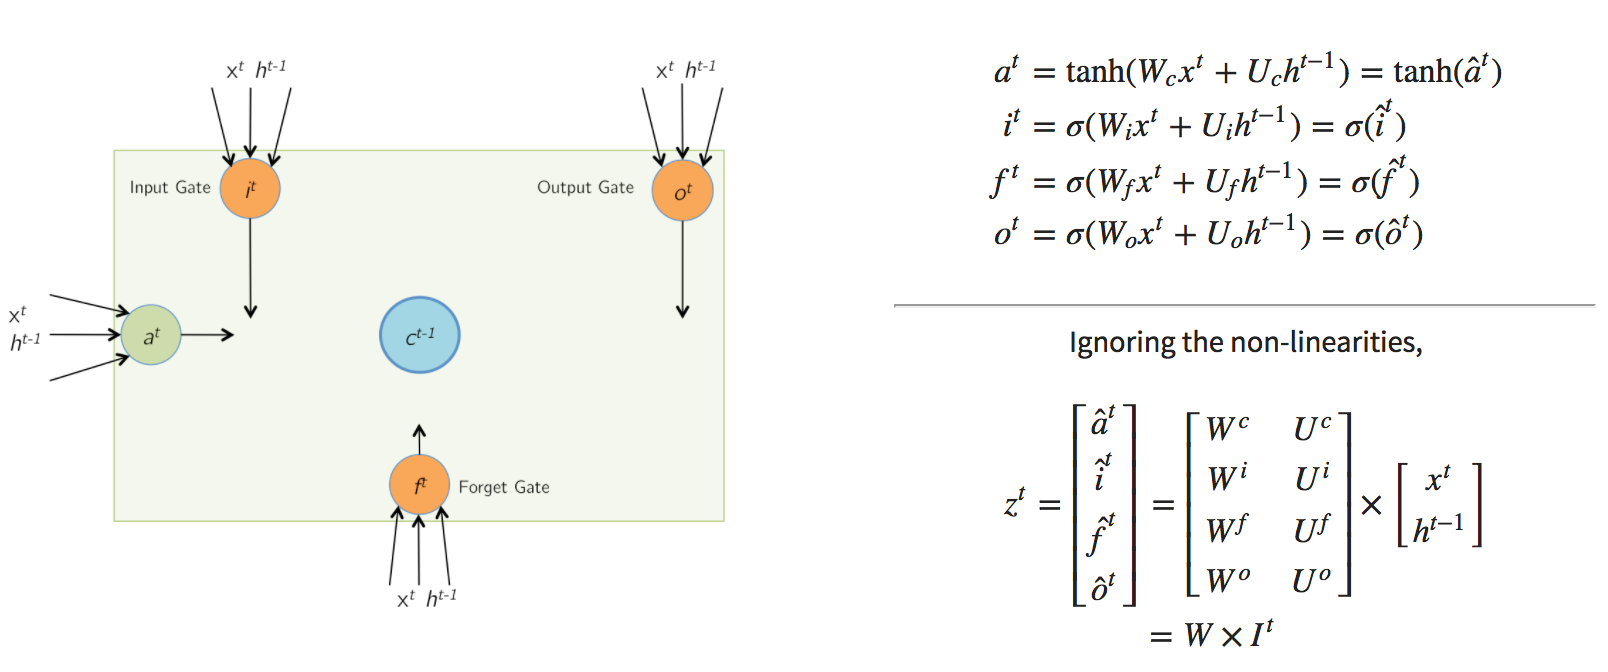
\includegraphics[width=1.0\textwidth]{lstm-input-gate-computation.png}
  \end{figure}
\end{frame}

\begin{frame}[fragile]{前向传播:状态更新}
  \begin{figure}
    \centering
    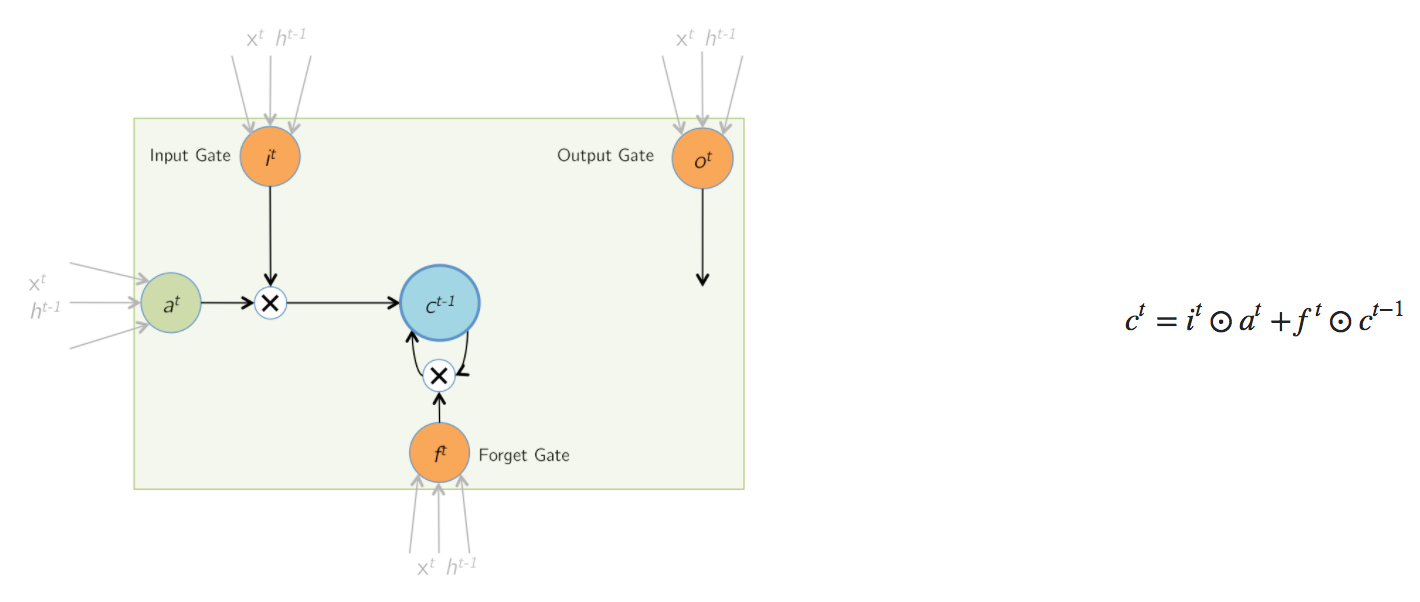
\includegraphics[width=1.0\textwidth]{lstm-update-cell.png}
  \end{figure}
\end{frame}

\begin{frame}[fragile]{前向传播:状态更新}
  \begin{figure}
    \centering
    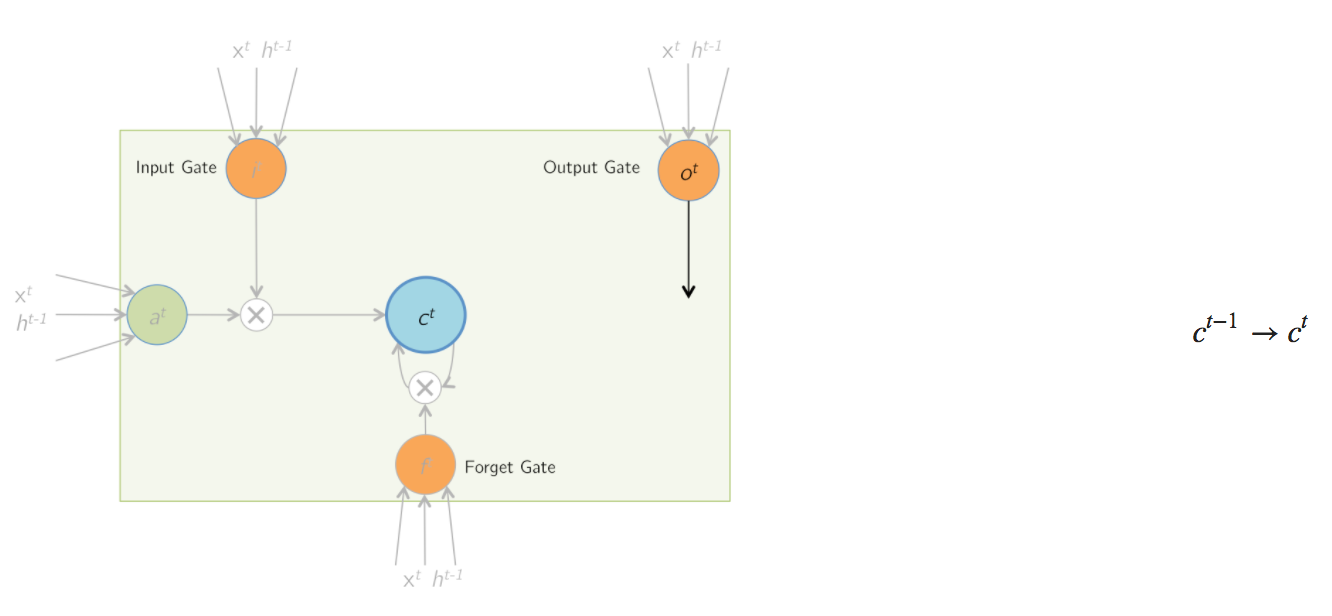
\includegraphics[width=1.0\textwidth]{lstm-update-cell-2.png}
  \end{figure}
\end{frame}

\begin{frame}[fragile]{前向传播:输出}
  \begin{figure}
    \centering
    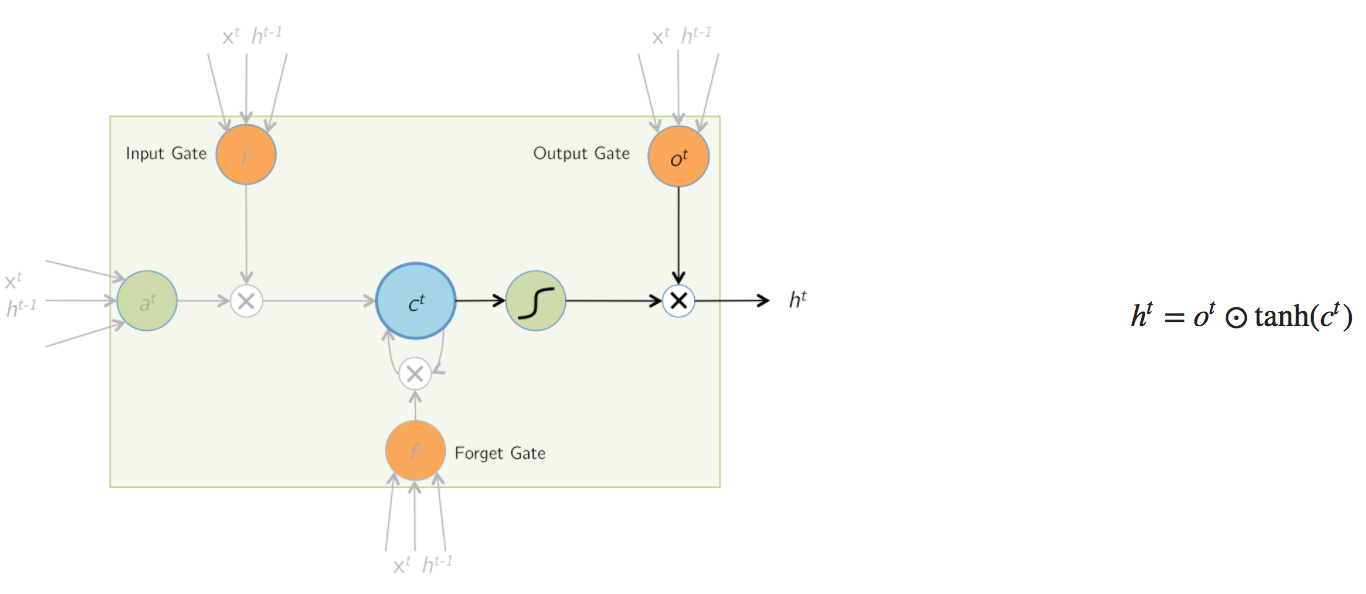
\includegraphics[width=1.0\textwidth]{lstm-output.png}
  \end{figure}
\end{frame}

\begin{frame}[fragile]{前向传播}
  \begin{figure}
    \centering
    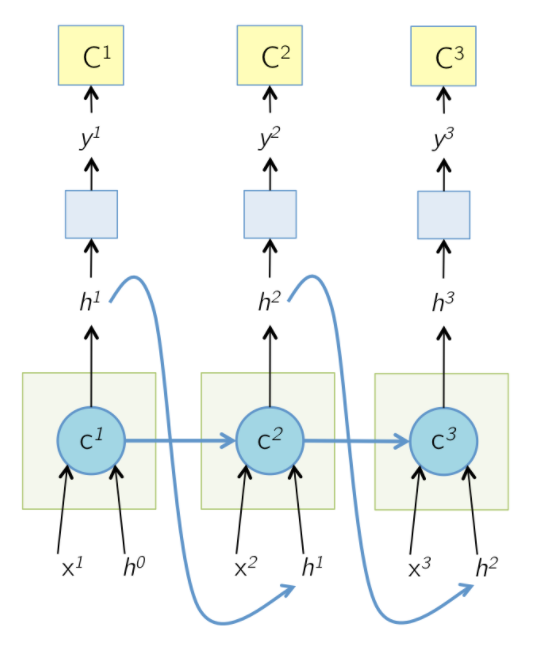
\includegraphics[width=0.5\textwidth]{lstm-unrolled_forward.png}
  \end{figure}
\end{frame}

\begin{frame}[fragile]{反向传播}
  \begin{figure}
    \centering
    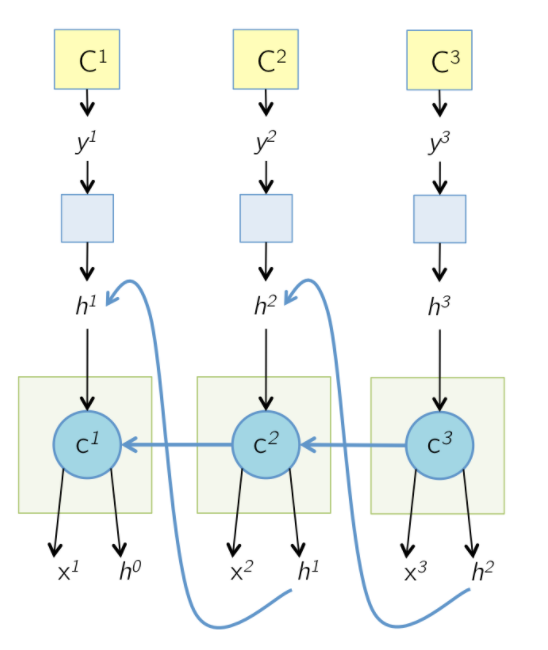
\includegraphics[width=0.5\textwidth]{lstm-unrolled_backward.png}
  \end{figure}
\end{frame}


\begin{frame}[fragile]{反向传播}
  \begin{figure}
    \centering
    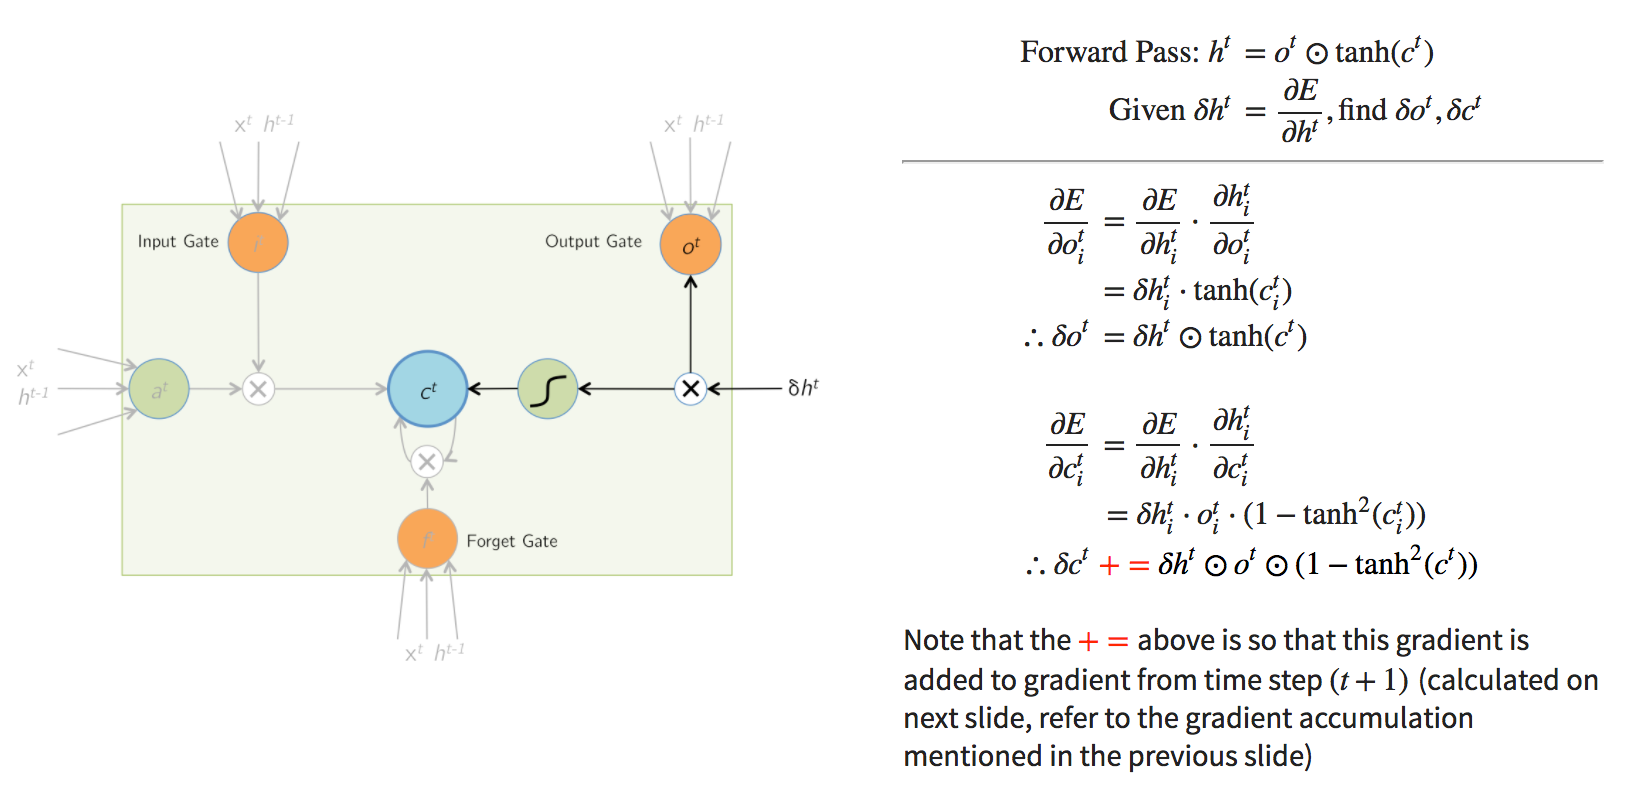
\includegraphics[width=1.0\textwidth]{lstm-bp-1.png}
  \end{figure}
\end{frame}


\begin{frame}[fragile]{反向传播}
  \begin{figure}
    \centering
    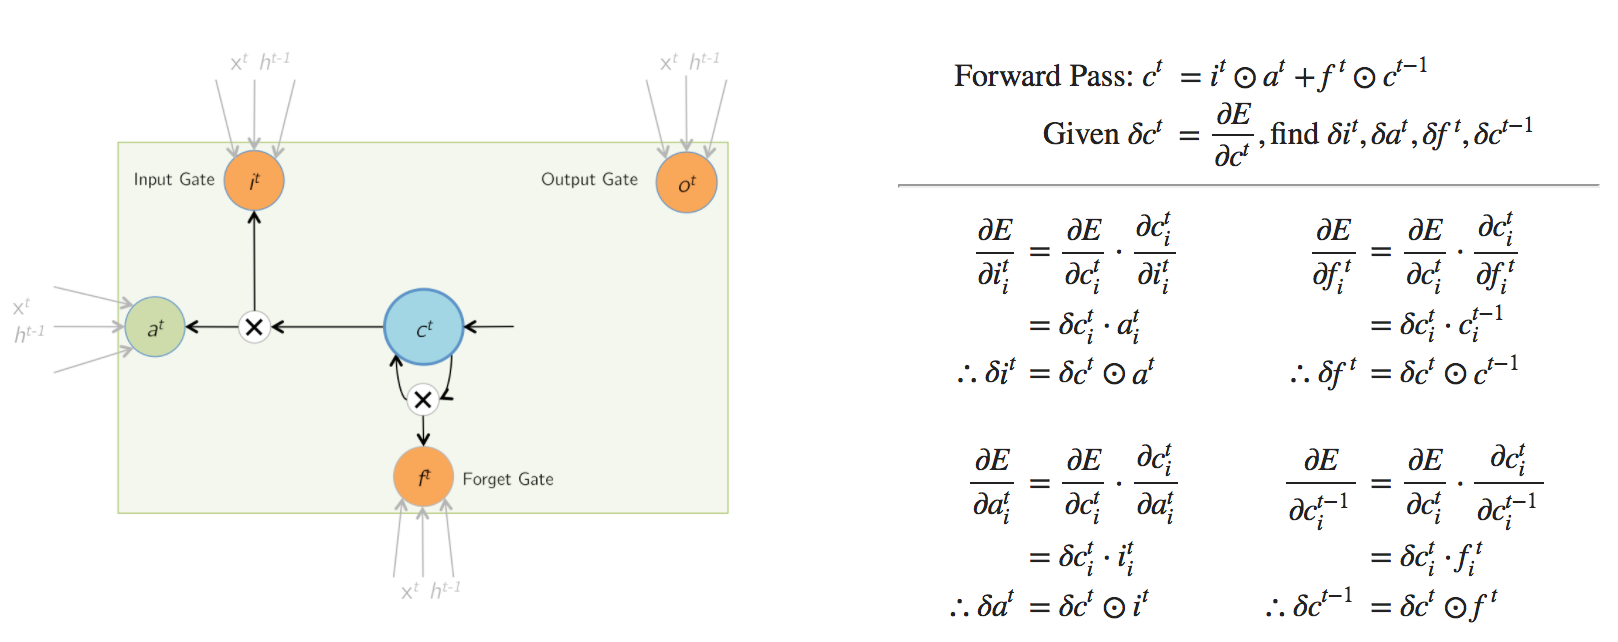
\includegraphics[width=1.0\textwidth]{lstm-bp-2.png}
  \end{figure}
\end{frame}


\begin{frame}[fragile]{反向传播}
  \begin{figure}
    \centering
    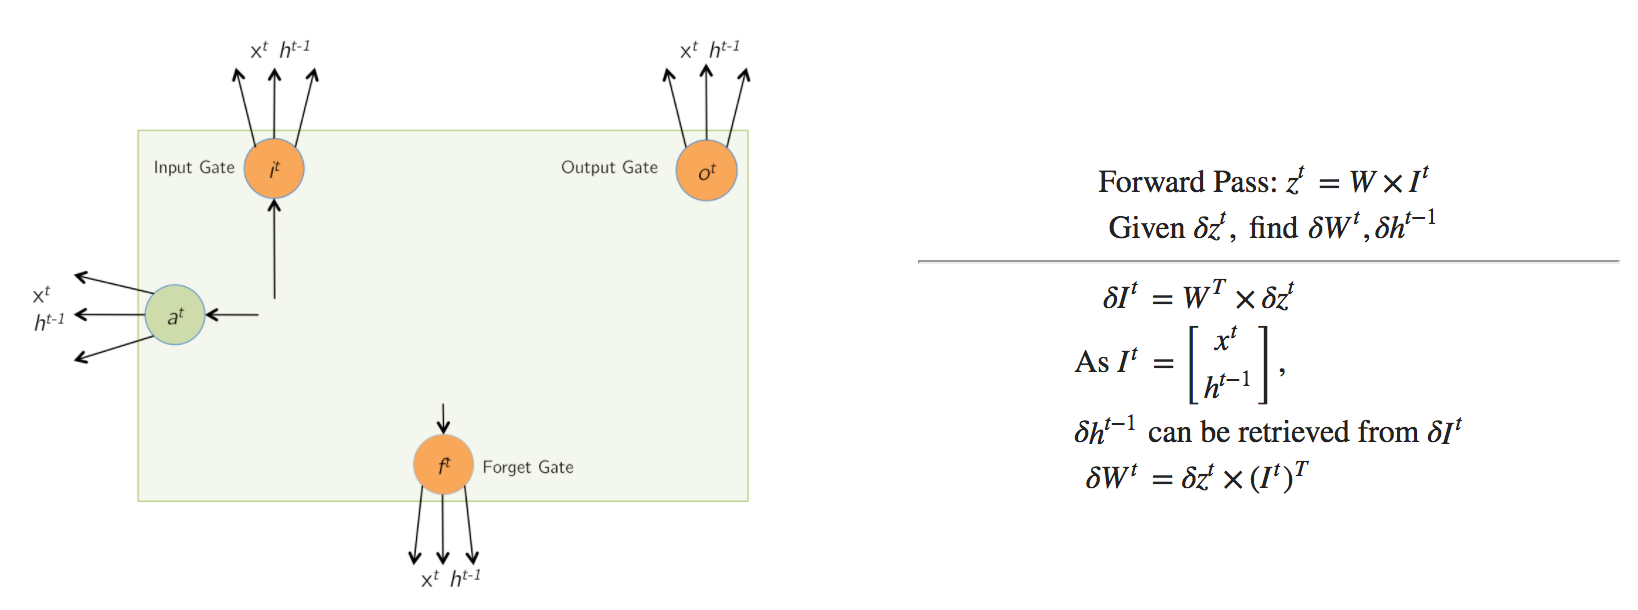
\includegraphics[width=1.0\textwidth]{lstm-bp-3.png}
  \end{figure}
\end{frame}


\begin{frame}[fragile]{反向传播}
  \begin{figure}
    \centering
    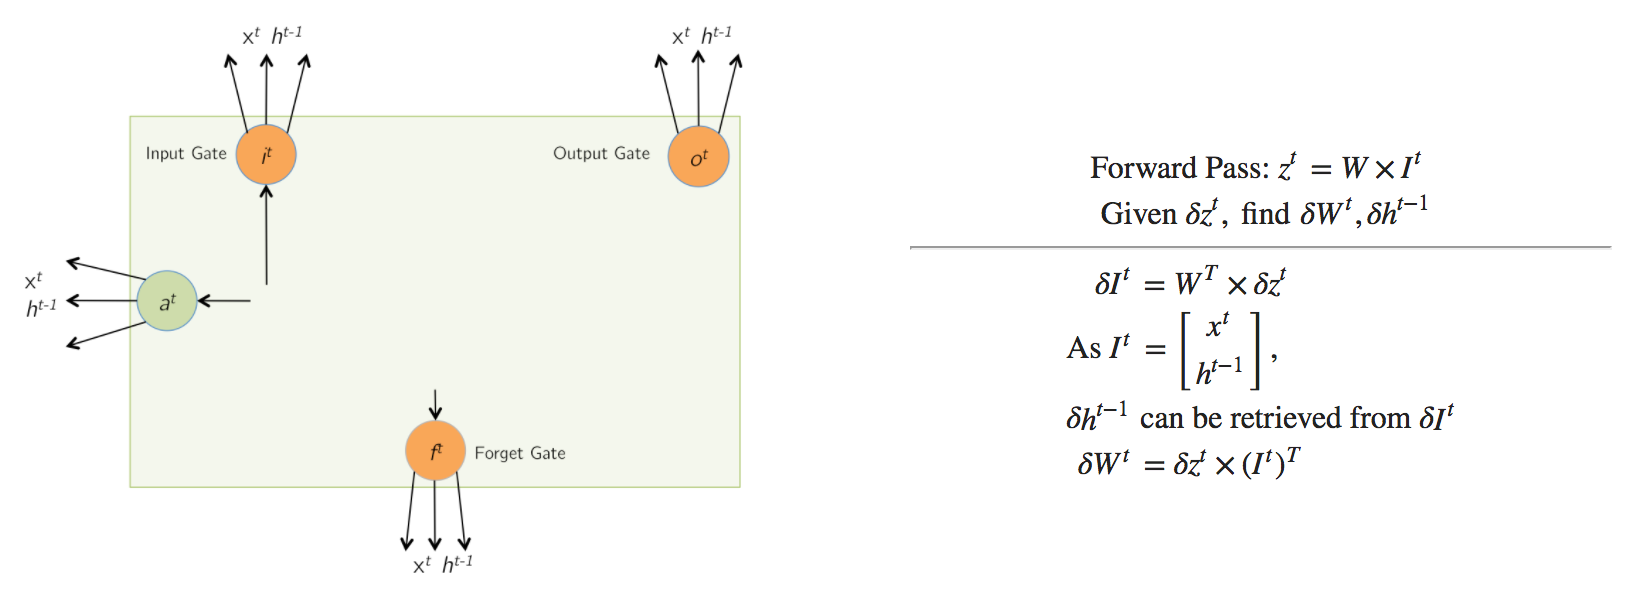
\includegraphics[width=1.0\textwidth]{lstm-bp-4.png}
  \end{figure}
\end{frame}


\subsection{变种}

\begin{frame}[fragile]{变种1}
  \begin{figure}
    \centering
    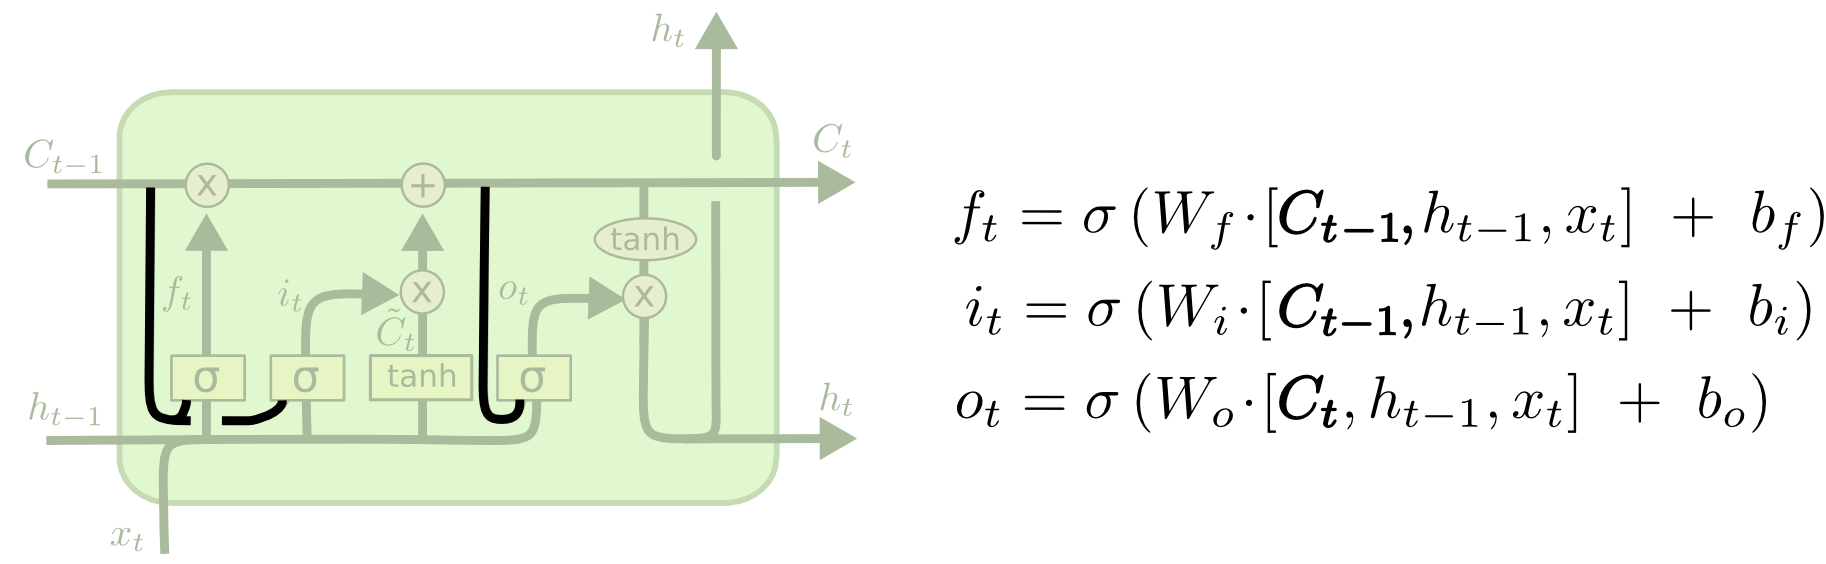
\includegraphics[width=0.9\textwidth]{LSTM3-var-peepholes.png}
  \end{figure}
\end{frame}

\begin{frame}[fragile]{变种2}
  \begin{figure}
    \centering
    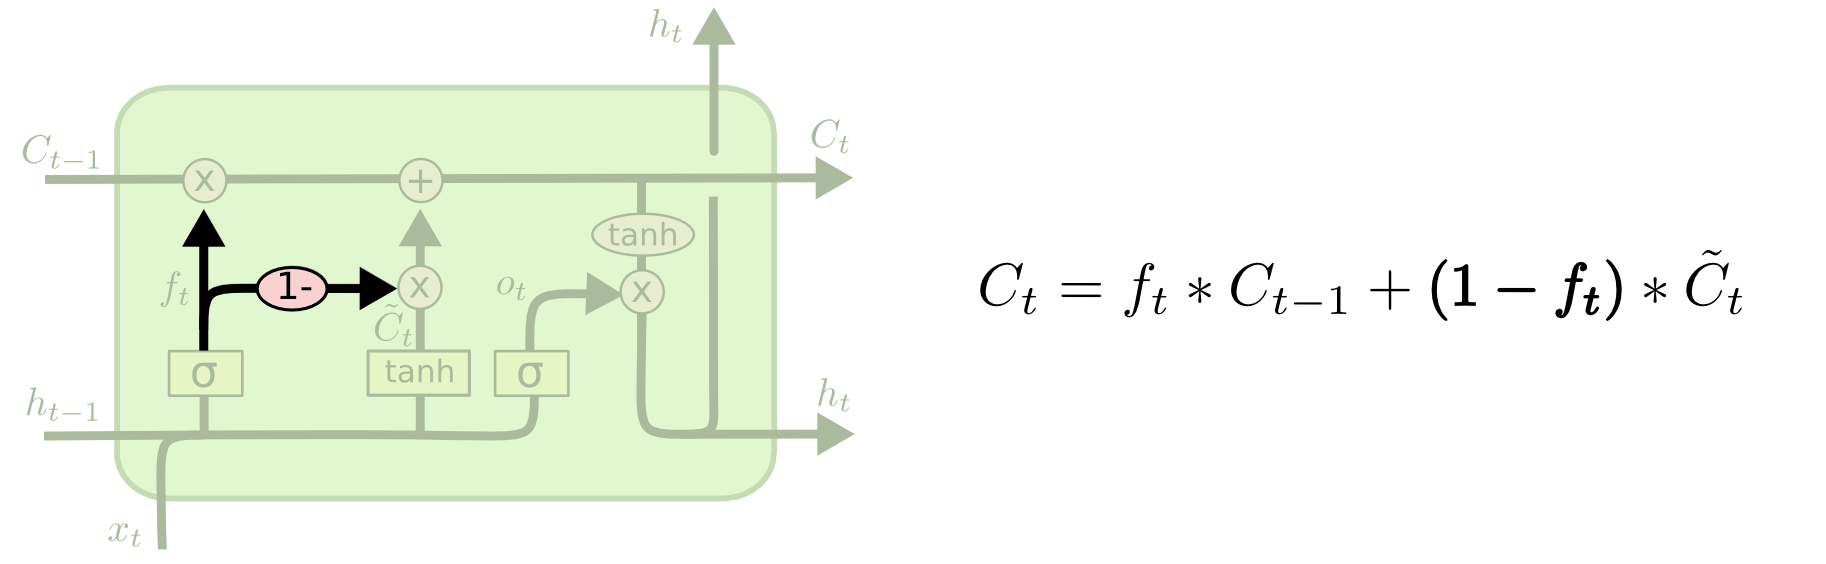
\includegraphics[width=0.9\textwidth]{LSTM3-var-tied.png}
  \end{figure}
\end{frame}

\begin{frame}[fragile]{变种3:GRU}
  \begin{figure}
    \centering
    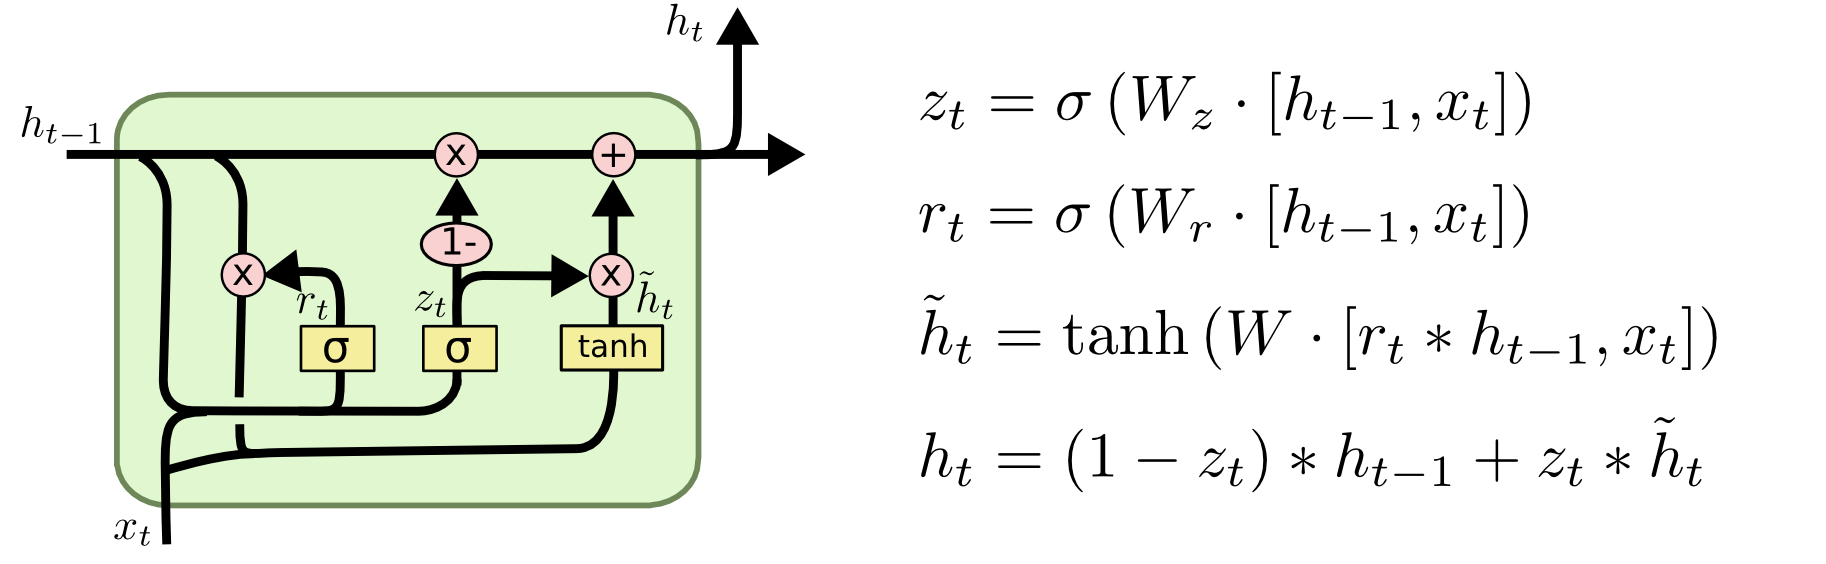
\includegraphics[width=0.9\textwidth]{LSTM3-var-GRU.png}
  \end{figure}
\end{frame}
